\chapter{Write Back}


\begin{figure}
\caption{Write Back}\label{fig:wb}
\begin{center}
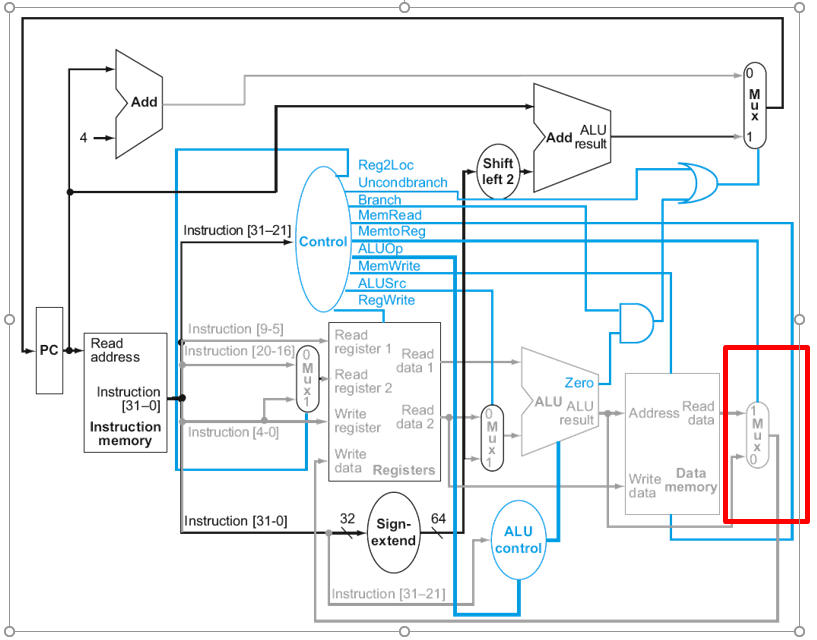
\includegraphics[width=\textwidth]{../images/writeback_stage.png}
\end{center}
\end{figure}

\WrapBarrier

\section{Mux}
This stage consists on only one item, a mux to select between the output of memory and the output of the ALU.  The control is the MemtoReg control line, see Fig~\ref{fig:wb}.  Since the mux has already been tested it does not need a testbench.  The stage thus has only 3 inputs (2 data and 1 control) and one output, the result.

\section{Datapath}
You are ready to assemble the full non-pipelined datapath shown in Fig~\ref{fig:datapath}.  To do this, you will need to combine all 5 stages into datapath.v.  Stages include:
\begin{enumerate}
\item iFetch
\item iDecode
\item iExecute
\item iMemory
\item iWriteBack
\end{enumerate} 

Verify by running your set of instructions in instrData.data and testing the output.  Pay particular attention to make sure that the Rd register is updated appropriately by R-Type and D-Type instructions.  You should no longer set write\_data in datapath.v.  Rather, you should connect write\_data from the WriteBack stage to the Decode stage.  For right now, keep pc\_src hard-coded to 0 in datapath.v.  Even though we could connect it now, our test instructions are not meant to run like a program and would yield strange results.  Each instruction should execute as expected according to your Expected Results Table.  Datapath.v should be your top-level Verilog file (no additional test drivers are necessary).

\begin{figure}
\caption{Full Non-Pipelined Datapath}\label{fig:datapath}
\begin{center}
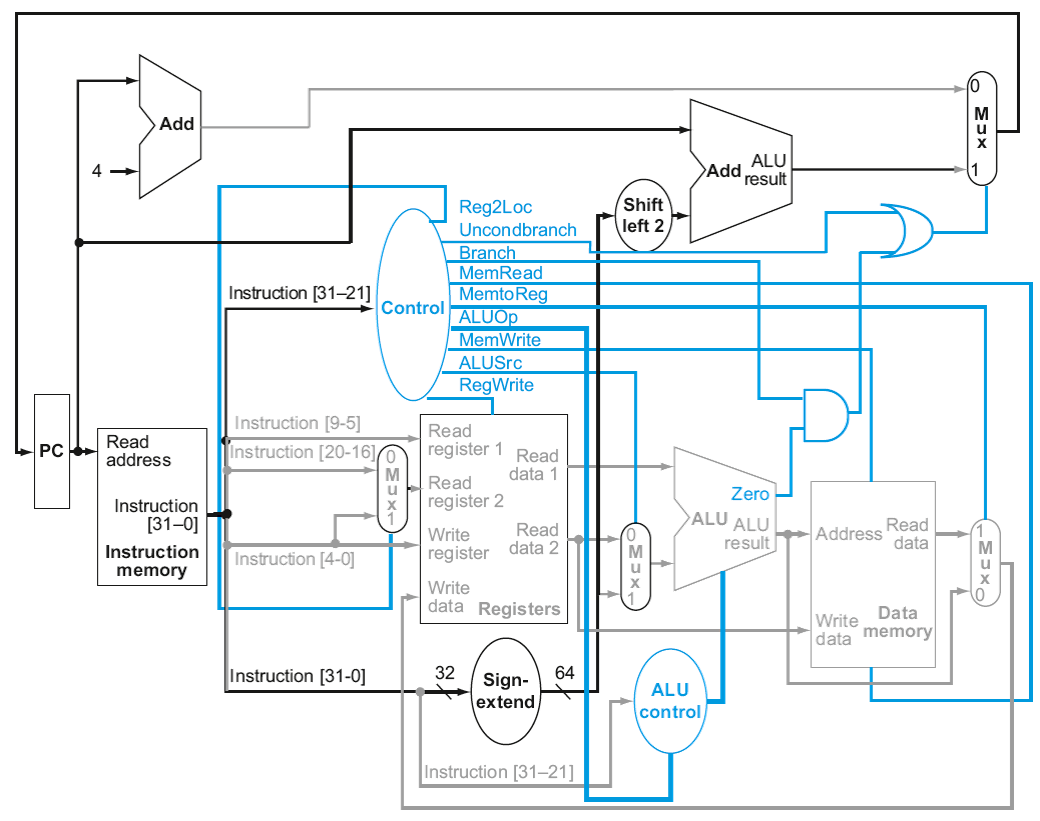
\includegraphics[width=\textwidth]{../images/non_pipelined_datapath.png}
\end{center}
\end{figure}

\section{Your Assignment Part 1}

You are to:
\begin{enumerate}
\item Create the Writeback stage consisting of one Mux.
\item Integrate all five stages into the file datapath.v.
\item Update your Expected Results Table to include the iWriteBack stage.
\item Run simulations to verify that your results match your Expected Results table.   
\item Do not write up a lab report yet. There will be one final test to add before we submit it.
\end{enumerate} 

\section{Division}
To further verify your datapath operation, you should create a new set of datafiles to implement the division code shown below.  You should first write assembly code, then translate it into binary.  One restriction is that the only non-zero value in your regData.data should be X22, which can be used as the base address for the array A.  Otherwise, all other data must be loaded from memory via the ramData.data and LDUR commands.  Please pay attention to the comments in division.c.

\Verilog{C code for doing simple division.}{code:division}{../code/division.c}

\begin{figure}
	\caption{Full Non-Pipelined Datapath}\label{fig:datapath}
	\begin{center}
		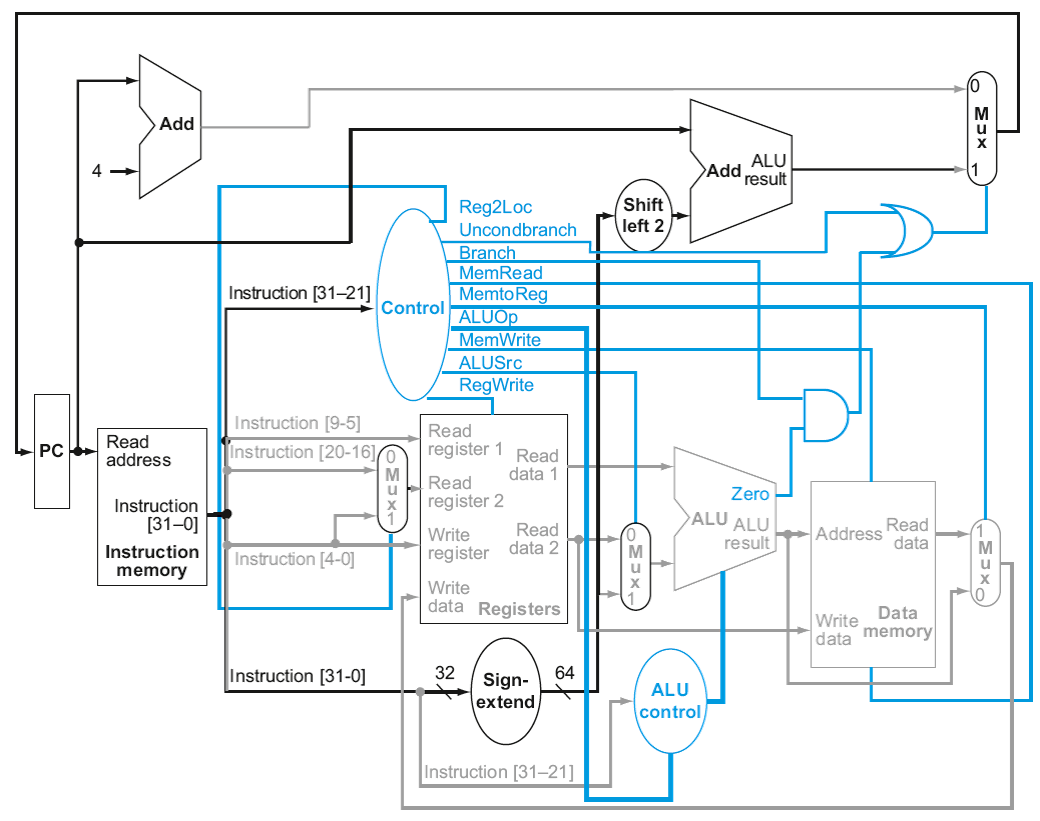
\includegraphics[width=\textwidth]{../images/non_pipelined_datapath.png}
	\end{center}
\end{figure}

\section{Your Assignment Part 2}

You are to:
\begin{enumerate}
	\item Implement the assembly and binary code for the Division C Code shown above.
	\item Verify that the divison works correctly.
	\item Write up a lab report according to the LabN format.
\end{enumerate} 